\documentclass[letterpaper,11pt,titlepage]{article}
\usepackage{authblk}
\usepackage{graphicx}
\usepackage{subcaption}
\usepackage{booktabs}
\usepackage[margin=0.5in]{geometry}
\usepackage[T1]{fontenc}
\usepackage{lmodern}
\usepackage{hyperref}
\usepackage{setspace}
\usepackage[UKenglish]{babel}
\usepackage{csquotes}
\usepackage{natbib}
\bibliographystyle{plainnat}
\onehalfspacing
\begin{document}
\title{The Aisled Hall at Mellor \\ An appraisal of the evidence}
\author{Day, Jonathan}
\author{Day, Philip}
\affil{Mellor Geophysics}
\maketitle
\begin{abstract}
Excavations at the Mellor Hilltop archaeological site have unearthed a set of post pits carved some 0.4-0.8m into the sandstone bedrock underlying about 0.5m of grass-covered topsoil. The 15 or so pits are probably the existing remainder of a set of 20 postholes, arranged in 4 rows each of 5 holes, overall dimension 10x12m. Various artefacts were found in the holes. These include 2 medieval iron arrowheads, pottery sherds, and one small wood remnant (C-14 dated to around 1200). These suggest a wooden building was constructed using the post-holes in around 1100 and destroyed approximately 200-250 years later. The archaeologists postulate that these discoveries demonstrate the existence of a wooden medieval aisled hall on this site over the relevant period.

This appraisal examines the archaeological evidence to reconstruct the most likely arrangement of 20 postholes. The various types of medieval construction which could be considered as contenders for this building are evaluated, and the hypothesis of an aisled hall is shown to be the most likely of the options. Assuming this assignment, the most likely structure of the original building is suggested, together with some speculations as to its purpose and occupancy, both at the time of construction and later alteration.
\end{abstract}
\section{Archaeological Data}
\subsection{Archaeological Evidence}
Excavations over the three-year period 2005-07 have uncovered evidence of a structure of early medieval origin in the vicinity of the Old Vicarage in Mellor. This evidence consists of four incomplete rows of five post pits (Figure \ref{fig:postholes}), each roughly circular and around 1 metre diameter {Figure \ref{fig:corner}, cut into the sandstone bedrock underlying the vegetable garden of the Old Vicarage, just to the north of Mellor Church (see Map and Diagram -- Figures \ref{fig:plan} \& \ref{fig:layout}, respectively).

The overlying topsoil, depth around 50 cm and extending down to the bedrock, has been cultivated for many years, whilst the surface of the bedrock itself is extensively fractured. On excavation, the post pits were found to be filled with soil and a mixture of small and large stones; in many cases there was evidence (discolouring) of a post pipe (Figure \ref{fig:postpipe}) around 40-45cm in diameter within the larger post pit. Inside and immediately around these pits, two medieval iron arrowheads have been found, along with early medieval pottery sherds and a fragment of wood which has been dated to between the 11th and 12th centuries. In the middle of the arrangement of post pits there is an area that appears to have been exposed to a considerable amount of heat over a long period of time, which could be the remains of a fireplace.

\begin{figure}
	\centering
	\begin{subfigure}[b]{0.30\textwidth}
		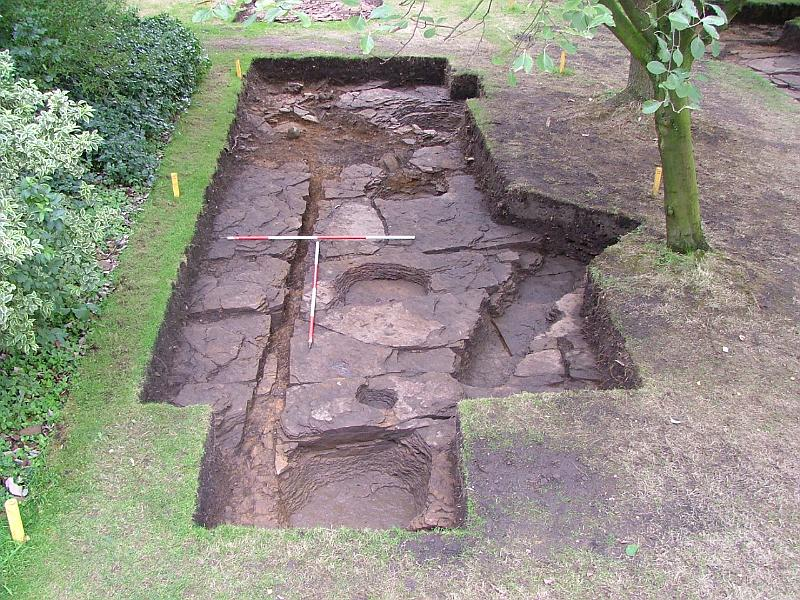
\includegraphics[width=\textwidth]{DSCF2859}
		\caption{Row of postholes with scale}
		\label{fig:postholes}
	\end{subfigure}
	\begin{subfigure}[b]{0.30\textwidth}
		\includegraphics[width=\textwidth]{pitpostpipe}
		\caption{Posthole with postpipe}
		\label{fig:postpipe}
	\end{subfigure}
	\begin{subfigure}[b]{0.30\textwidth}
		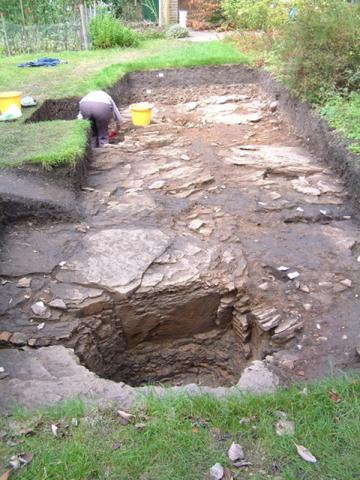
\includegraphics[width=\textwidth]{Mellor_hall}
		\caption{Postholes being excavated}
		\label{fig:corner}
	\end{subfigure}
	\begin{subfigure}[b]{0.45\textwidth}
		\includegraphics[width=\textwidth]{mapgrid}
		\caption{Excavation plan showing post pits assigned to the medieval period}
		\label{fig:plan}
	\end{subfigure}
	\begin{subfigure}[b]{0.45\textwidth}
		\includegraphics[width=\textwidth]{fullgrid}
		\caption{Diagrammatic layout of the post pits, with dimensions in metres to the centres of each post pit}
		\label{fig:layout}
	\end{subfigure}
	\caption{Archaeological excavations at the Old Vicarage, Mellor Hilltop}\label{fig:excavations}
\end{figure}

\subsection{Excavations Report}
The 2006 Excavation Report (section 4.2.7) gives details of post holes excavated in trench 34 (5 in 2005) and trench 43 (7 in 2006). These have been assigned to the medieval period (11th to 14th Centuries) on the basis of various artefacts discovered in the post holes (pottery, iron arrowheads, wood fragment C14 dated). Although some post holes are missing from the set of observations, there are plausible reasons for this, and it has been suggested that the post hole array is evidence of a wooden building supported by 4 rows of 5 posts, overall dimension approximately 11.8m long (roughly North-South) by 10.1m wide. The gap between the two centre rows (4.1m) is wider than the gaps between the outer rows (average 3.0m). These facts are taken as evidence for the existence of a medieval Aisled Hall, of which there are several similar (but not identical) examples in England, mostly in the southern counties. The Hall may have been constructed in the 11th Century, and was probably destroyed in the late 14th Century.

A number of discrepancies with this explanation are noted: the apparent absence of at least 3, possibly 5, post holes; the poor alignment of many of the post holes with a regular grid and the severe misalignment of post holes in the most westerly row. None-the-less, informed archaeological opinion is that the Aisled Hall assignment is correct.

Where feature numbers are given, they refer to the feature numbers in the 2006 Excavations Report.

\subsection{Measurements}
Overall foundation width: 11.7m; Row separations, 3.1, 4.1, 2.9m (average outer rows, 3.0m)\\
Overall foundation length: 11.8m; Post column separations, 2.9, 3.0, 2.7, 3.2m (average, 2.95m)\\

Of a hypothetical full complement of 20 postholes, 6 are not observed, in 2 cases (8, 10) because trees prevented excavation. In the other 4 cases (13, 16, 18, 19), the ground was excavated but no posthole was seen. It is possible that fragmentation of the bedrock obscured evidence of posthole remnants, or equally possible that no posthole existed at these positions. In two cases where a posthole did exist (7, 12), a shallower feature was identified adjacent to the pit. In the case of (12), this may be a distinct post pit but no posthole was identified for it.

\begin{figure}
	\centering
	\begin{subfigure}[b]{0.45\textwidth}
		\includegraphics[width=\textwidth]{schematic}
		\caption{Idealised diagram of observed postholes}
		\label{fig:schematic}
	\end{subfigure}
	\begin{subfigure}[b]{0.45\textwidth}
		\includegraphics[width=\textwidth]{identifiers}
		\caption{Numbered positions}
		\label{fig:identifiers}
	\end{subfigure}
	\caption{Summary (all measurements are averages and to posthole centres)}\label{fig:measurements}
\end{figure}

\begin{table}[]
	\small
	\centering
	\caption{Table showing observed postholes and characteristics}
	\label{characteristics}
	\begin{tabular}{|p{1.25cm}|p{1.25cm}|p{1.25cm}|p{1cm}|p{1cm}|p{1.5cm}|p{4.5cm}|p{4cm}|}
		\toprule
Posthole & Trench No. & Feature No. & Dia. /cm & Depth /cm & Post pipe dia. /cm & Artifacts & Notes \\
		\midrule
1  & 34 &       & 100       &    &    &                                                                                    & circular. very deep              \\ \hline
2  & 34 &       & 100 x 120 &    &    & wood fragment, C14 date 1000-1250 (found in one of the postholes 1-5)           & rectangular                      \\ \hline
3  & 34 &       & 90        &    &    &                                                                                    & circular                         \\ \hline
4  & 34 &       & 100       &    &    &                                                                                    & circular                         \\ \hline
5  & 34 &       & 120       &    &    &                                                                                    & circular                         \\ \hline
6  & 43 & [015] & 160       & 60 & 45 &                                                                                    & circular                         \\ \hline
7  & 43 & [003] & 160       & 67 &    & 12 sherds medieval pottery. Fe arrowhead. 1 jar (C11-C13). 1 grindstone (C12-C14). & circular                         \\ \hline
8  &    &       &           &    &    &                                                                                    & tree prevented excavation        \\ \hline
9  & 43 & [010] & 124       & 40 & 45 & pottery (C12-C14)                                                                  &                                  \\ \hline
10 &    &       &           &    &    &                                                                                    & tree prevented excavation        \\ \hline
11 & 43 & [144] & 75 x 120  &    & 30 &                                                                                    & oval                             \\ \hline
12 & 43 & [024] & 137       & 81 & 35 & 1 jar (C11-C13)                                                                    & circular                         \\ \hline
13 &    & [001] &           &    &    &                                                                                    & not observed in excavated ground \\ \hline
14 &    & [032] &           &    &    &                                                                                    &                                  \\ \hline
15 &    & [082] &           &    &    &                                                                                    &                                  \\ \hline
16 &    &       &           &    &    &                                                                                    & not observed in excavated ground \\ \hline
17 & 43 & [123] & 160       & 56 & 40 &                                                                                    & circular. Possibly [103]         \\ \hline
18 & 33 &       &           &    &    &                                                                                    & not observed in excavated ground \\ \hline
19 & 33 &       &           &    &    &                                                                                    & not observed in excavated ground \\ \hline
20 & 33 &       &           &    &    &                                                                                    &                                  \\ \hline
		\bottomrule
	\end{tabular}
\end{table}

\subsection{Hypothesis}
The archaeological hypothesis (reference: Annual Reports \Citet{exc2005,exc2006,exc2007}) is that these observations, taken together, strongly suggest the original presence of a medieval Aisled Hall, of four bays, supported on wooden posts. The postulated date of construction is towards the end of the 12th Century, with demolition around the middle of the 14th Century, these dates being based on the nature of the various artefacts found in the post pits, and the C-14 date for the wooden remnant.
\section{Historical Data}
\subsection{Historical Evidence from the Medieval Period} 
There is very little documentary evidence of what was happening in Mellor during the Norman and Plantagenet periods. A reference to Ludworth exists in the Domesday book, but there is no clear indication of just how large a territory Ludworth was at that time or, indeed, where in that territory any of the structures listed actually were. There are also references which suggest part or all of Mellor was within the Royal Forest of the Peak. 

A stone church almost certainly existed on the present hilltop site at Mellor (Figure \ref{fig:mellorchurch}) in the 12th Century, and quite possibly parts had been there for several centuries; for example, the base of the tower at the west end (Figure \ref{fig:churchtower}) is thought to date from around or before 1100. Some of the furnishings inside the present church (for example, the font and pulpit, Figures \ref{fig:baptismfont} and \ref{fig:pulpit}) may date from Saxon times, suggesting the existence of an earlier (probably wooden) church on or around the same site. The pulpit is carved from a single piece of oak.

It is, therefore, conceivable that the postulated Aisled Hall was, during the relevant period, the residence of the local priest. It is also possible that the structure originates from an earlier period, and was originally the church itself, possibly later (after the construction of a stone church) becoming the priest's residence.

\begin{figure}
	\centering
	\begin{subfigure}[b]{0.3\textwidth}
		\includegraphics[width=\textwidth]{mellorchurch}
		\caption{The church from above}
		\label{fig:mellorchurch}
	\end{subfigure}
	\begin{subfigure}[b]{0.3\textwidth}
		\includegraphics[width=\textwidth]{churchtower}
		\caption{The tower}
		\label{fig:churchtower}
	\end{subfigure}
	\begin{subfigure}[b]{0.3\textwidth}
		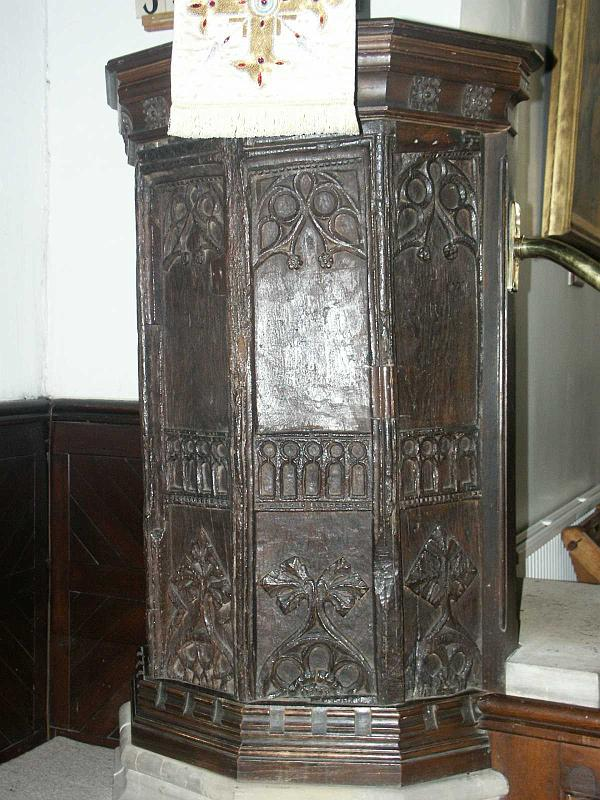
\includegraphics[width=\textwidth]{pulpit}
		\caption{The pulpit}
		\label{fig:pulpit}
	\end{subfigure}
	\caption{St. Thomas' church in Mellor}\label{fig:thomas}
\end{figure}

\section{Comparisons With Other Structures}
\subsection{Pre-Norman Structures}
It is necessary to first examine if the base plan is that of a medieval hall, for a number of reasons. First, their crude form and severe damage is not easy to explain, given that much older postholes exist in much better condition and Norman craftsmen were highly skilled. Secondly, there are a large number of structures either recorded historically or for which there is indirect archaeological evidence for which no archaeology has been definitely found. It is necessary to verify that an unidentified structure is not one of them. Thirdly, the extensive reuse of the site means that opportunistic reuse of features cannot be ruled out. Ultimately, any deductions based on the floor plan are valid only if the floor plan can be directly related to the medieval structure that made use of it.

The site in Mellor has revealed occupation from the Mesolithic into Saxon times. In order to thoroughly examine the possibilities, it is necessary to examine architectures prior to the Norman period. In the event that the site was re-used in later times, it would be difficult to eliminate any given possibility from having ever existed. However, it is certainly possible to determine if the postholes conform to any known prior architecture. In the case of Saxon buildings, this is fairly straight-forward. Saxon architecture, insofar as it is known, falls into two broad types -- stone buildings and wooden buildings that rested on the ground.

As far as can be determined, Saxons did not construct buildings using posts secured deep into the ground. A similar argument can be presented for Norse architecture. From this, we can say with some certainty that whether or not such buildings existed in the Mellor region, they did not produce any of the post-holes.

Going back further, the Romano-British phase does not appear to have been substantially different from the Iron Age phase in architecture, where round-houses dominated the scene. Round-houses did indeed require post-holes, but the layout is quite distinct. There is no significant evidence of rectilinear architecture in Britain from there back until Neolithic times. However, the few surviving examples of rectilinear Neolithic post-holes indicate buildings supported along a central ridge, with small, closely-spaced post-holes running down the centre of the structure. The existing post-holes in Mellor do not fit this design and the space between the existing post-holes lack any evidence of the smaller indentations required for this hypothesis. Known Mesolithic houses in Britain used a circular arrangement of posts.

From this, it can be concluded that whatever earlier structures may have existed, they are not the cause of the post-holes either in their current state or in some earlier form. Therefore, their highly fragmented state and rough form is not a product of reuse or a greater period of time, and we can directly use known medieval floor plans and existing halls as a basis for describing the hall at Mellor.

\begin{figure}
	\centering
	\begin{subfigure}[b]{0.3\textwidth}
		\includegraphics[width=\textwidth]{bylany}
		\caption{Neolithic Longhouse at Bylany}
		\label{fig:bylany}
	\end{subfigure}
	\begin{subfigure}[b]{0.3\textwidth}
		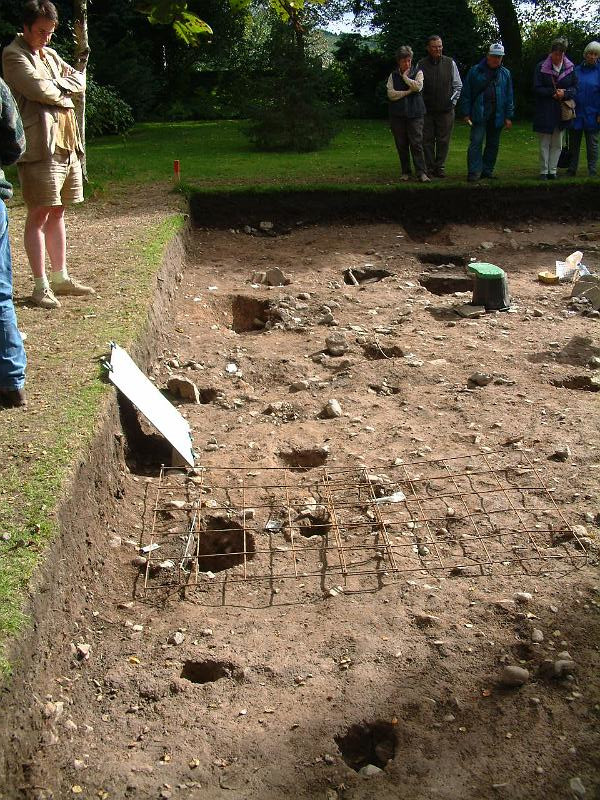
\includegraphics[width=\textwidth]{DSCF1510}
		\caption{Round-house Postholes}
		\label{fig:roundhouse}
	\end{subfigure}
	\caption{Pre-Norman Postholes}\label{fig:prenorman}
\end{figure}


\subsection{English Medieval Halls}
Architecture in medieval England was fairly diverse and included merchant's houses, ``King John's Houses'', First-Floor Halls, Aisled Halls, Spere Truss Halls and Great Halls, to name but a few. In order to successfully determine what has been found in Mellor, it is necessary to first eliminate those possibilities that do not fit the evidence as it has so far been determined. The terminology in this paper is consistent with the usage introduced in The English Medieval House (Wood, Margaret) except where otherwise noted. Examples follow current classification within this structure.

\subsection{Merchant's Houses and King John's Houses}
The first two possibilities are the easiest to eliminate. There appears to be a fair amount of documentary evidence that merchant's houses and ``King John's Houses'' were built from stone, whereas the building in Mellor has post holes, implying a wooden construction. This was not through a lack of availability of stone, as the local gritstone was certainly used in the making of a number of artefacts such as the font currently located in Mellor Church (Figure \ref{fig:baptismfont}) and the two pillars that comprise the Picking Rods a short distance north-east of Mellor (Figure \ref{fig:pickingrods}); This does not eliminate the possibility of there having been a merchant house somewhere on the site, it merely shows that the building in question was of a different design.

\begin{figure}
	\centering
	\begin{subfigure}[b]{0.3\textwidth}
		\includegraphics[width=\textwidth]{fontchurch}
		\caption{Sandstone Saxon baptismal font}
		\label{fig:baptismfont}
	\end{subfigure}
	\begin{subfigure}[b]{0.3\textwidth}
		\includegraphics[width=\textwidth]{robhoodpick2}
		\caption{Robin Hood Picking Rods}
		\label{fig:pickingrods}
	\end{subfigure}
	\caption{Sandstone Artifacts dated to between the 9th and 11th centuries}\label{fig:saxons}
\end{figure}

\subsection{First-Floor Halls}
First-Floor Halls, also known as Raised Halls, were built between the 11th and 13th centuries, which would place them in the correct period. These Halls were designed to have the ground floor as a vaulted open area, with the Hall itself on the first floor. This appears to have been primarily designed defensively, following the design of keeps in having living quarters raised from the ground floor. However, all known examples of First-Floor Halls use stone for the ground floor, as indeed would be a necessity if the halls had a defensive purpose. (\Citet{medievalhouse,firstfloorhall}) Where wood is suspected to have been used, it is believed to have been used on the first floor and perhaps on the stairs reaching it. The Bayeux Tapestry seems to depict a wooden Hall raised on a motte, or earth mound. So far, there is no suggestion of there having been an earth mound at the Mellor location although, given the heavy re-use of the site, this would be hard to prove. 

Scolland's Hall, Richmond Castle (Figure \ref{fig:scolland}), is recognized as an example of a First Floor Hall. (\Citet{scollandshall})

Another characteristic of First-Floor Halls was that they were generally divided into two sections, a large section for general use and a smaller section, referred to as the Solar, for the owner's private use. The partition sometimes, but not always, appears on the ground floor as well as the first floor. Even where the partition itself does not appear on the ground floor, the ground floor construction is different beneath the solar than for the rest of the Hall. There is no evidence for such a difference at the Mellor site.

Overall, although this possibility cannot be totally disproved, there is nothing that lends itself to suggest that the building was a First-Floor Hall and sufficient indications to suggest otherwise that this possibility must also be set aside.

\subsection{Aisled Halls}
As with First-Floor Halls, Aisled Halls were also relatively common in England between the 11th and 13th centuries (reference). These Halls were generally fairly wide buildings and used lines of posts to hold up the roof. In cases in which the Halls had multiple floors, this technique was also used to hold up the ceiling. Aisled Halls were typically built at the ground floor level, and varied in size, shape, and mode of construction. Some were built of stone, or stone and brick, and many of these are still in existence (see Figure \ref{fig:oakham} for an example). But many were built entirely of wood, and some of these are also in existence (see Figures \ref{fig:tymawr} \& \ref{fig:greatbarn}). The largest known Aisled Hall had support posts two feet square set in holes six feet deep. This would in principle allow for these posts to be fifty or sixty feet high. The shape varied from being almost square to being three or four times as long as wide, although the design did not place any real limit on the length of the structure.

\begin{figure}
	\centering
	\begin{subfigure}[b]{0.3\textwidth}
		\includegraphics[width=\textwidth]{oakham}
		\caption{Oakham Castle}
		\label{fig:oakham}
	\end{subfigure}
	\begin{subfigure}[b]{0.3\textwidth}
		\includegraphics[width=\textwidth]{TyMawr015}
		\caption{Ty Mawr}
		\label{fig:tymawr}
	\end{subfigure}
	\begin{subfigure}[b]{0.3\textwidth}
		\includegraphics[width=\textwidth]{Harmondsworth}
		\caption{Harmondsworth Great Barn}
		\label{fig:greatbarn}
	\end{subfigure}
	\caption{Extant Aisled Halls}\label{fig:aisled}
\end{figure}

The general design was relatively straight-forward and conformed to obvious engineering principles (see Figures \ref{fig:burmington}, \ref{fig:barn} \& \ref{fig:rafters}), although at the time the ``principles'' would no doubt have been practical rather than theoretical. The inner two rows of posts supported transverse and longitudinal beams, and the latter formed the main support for the roof (and upper floor if it existed). The full weight of the central (main) section of the roof ultimately rested on these posts. The outer rows of posts, which would usually have been considerably shorter, allowing for the construction of two side ``aisles'' (e.g. typical of a medieval church), making the overall width of the hall considerably greater than the span of the central beam.

\begin{figure}
	\centering
	\begin{subfigure}[b]{0.65\textwidth}
		\includegraphics[width=\textwidth]{construction}
		\caption{Burmington Manor, east and west views}
		\label{fig:burmington}
	\end{subfigure}
	\begin{subfigure}[b]{0.45\textwidth}
		\includegraphics[width=\textwidth]{2dsmall}
		\caption{Barley Barn, Cressing and Harlowbury, Essex}
		\label{fig:barn}
	\end{subfigure}
	\begin{subfigure}[b]{0.45\textwidth}
		\includegraphics[width=\textwidth]{3small}
		\caption{Rafters}
		\label{fig:rafters}
	\end{subfigure}
	\caption{Construction of an Aisled Hall}\label{fig:construction}
\end{figure}

Larger buildings were divided into several segments, or bays, with different beams for each segment. Across and along each bay there would be horizontal beams that rested on top of the innermost support posts, and the longitudinal beams would support the ends of the rafters holding the central section of the roof. These rafters would meet at the centre ridge of the structure, although sometimes there were also vertical posts resting on the transverse beams to provide additional support for the roof. The roofs of the side aisles were sometimes supported on extensions of the central rafters, but more commonly the side aisles had separate rafters at a lower pitch than the main roof. The outer wall of the building would have been in line with the outer rows of posts. Usually, the outer wall rested on stone or rubble, but would not have been load-bearing. 

In earlier constructions, diagonal braces across the various right angles would have been used to provide rigidity, and later, arches between the support posts both across and down the Hall were used for this purpose. Eventually, the arch construction developed to the point that the two inner rows of posts became superfluous, and the ``Great Hall'' evolved (see below and Figure \ref{fig:greathall}).

The specific details, however, changed over the time such buildings were constructed. Surviving 11th century examples are often large and grandiose. 12th century Aisled Halls seem to have been more modest in size but heavily Gothic in character. Finally, 13th century designs appear to have been influenced more by practicality and functionality than appearance. The 13th century also saw the elimination of single posts being used for support, replacing them with four shafts arranged as a quatrefoil. Exceptions exist to all of these general descriptions, as might be expected, but they are frequently enough seen in the surviving examples to be useful as a guide.

Unlike the other Halls, the Aisled Hall was a very general-purpose design, used for temples and cathedrals, castle halls, country houses for the wealthy, assembly points for communities and barns for land owners and farmers. Indeed, modern farm barns are ultimately derived from the Aisled Hall design. For this reason, it is insufficient to know that a structure is simply an Aisled Hall, as there are many variations in design, nature and role. 

\subsection{Spere Truss Halls}
These are a derivative of the Aisled Hall, which appeared as advancements in roof technology improved. A Spere Truss Hall (Figure \ref{fig:althrey}) used a braced collar beam for the central span, eliminating the need for the posts within the Hall itself. Only the posts for the outer walls were required. These structures are 14th century, which is later than the carbon dating for the wood retrieved from the site, and would not have had post pits inside the structure as noted in Mellor. These Halls are mentioned because they were the only Aisled Hall derivative to be common in the north and west of England, but can be rejected on the grounds of period and design.

\subsection{The Great Hall}
During the 13th century, another new design was being developed which omitted interior support posts. These Great Halls (Figure \ref{fig:greathall}) used elaborate networks of beams and arches connecting to the outer wall to provide the support for the roof. Because the excavations in Mellor have revealed a central row of supports, the Great Hall can be immediately excluded from consideration. 

\begin{figure}
	\centering
	\begin{subfigure}[b]{0.3\textwidth}
		\includegraphics[width=\textwidth]{Richmond}
		\caption{First-Floor Hall, Richmond Castle}
		\label{fig:scolland}
	\end{subfigure}
	\begin{subfigure}[b]{0.3\textwidth}
		\includegraphics[width=\textwidth]{trusshall}
		\caption{Spere Truss Hall, Althrey Hall}
		\label{fig:althrey}
	\end{subfigure}
	\begin{subfigure}[b]{0.3\textwidth}
		\includegraphics[width=\textwidth]{greathall}
		\caption{Great Hall, Stirling Castle}
		\label{fig:greathall}
	\end{subfigure}
	\caption{Examples of Different Types of Hall}\label{fig:different}
\end{figure}

\section{The Hall at Mellor}
At Mellor, there have been four parallel rows of post pits excavated in total, each averaging about a metre across, with several rows revealing five post pits.  This would produce four equal bays, a design for which there are examples dating to the 12th and 13th centuries. This is still more suggestive than definitive, but it can reasonably be said that of the Hall types so far considered, the Aisled Hall is the best match for the information so far available.

However, as has already been noted, there were many different types of Aisled Hall, depending on the time of construction and the nature of its use. It is necessary to dig into the available information a little deeper to gain a better understanding. 

The first problem is determining if there is an existing Aisled Hall of roughly the same dimensions with the same number of posts and the same number of bays. In the first of the trenches excavated, there are five post pits, averaging 1 metre across and placed on average 2.65 meters apart. From the eastern line of post pits, the gap to the next line of pit posts is 3.4 metres. After that is a gap of 3 metres to the next post pits. The distance to the fourth row is not specified but may be taken as similar.

The foundations actually measure 11.8 x 11.7 metres, but it must be borne in mind that non-fortified Aisled Houses did not always terminate on a supporting post and several had an overhang with a wattle-and-daub outer wall, creating a half or full additional bay. This would allow for a building 14.45 x 14.7 metres in size.

Although the information is incomplete, it is sufficient for determining if anything similar has been found. In fact, there are several reasonably close matches. There are two castle Aisled Halls of the correct age, aisle count and width but greater than the maximum length of the Aisled Hall at Mellor. These are the Aisled Halls at Oakham Castle in Rutland and at Farnham Castle in Surrey. Both are dated to 1190. They have 4 bays, a total length of 20.1 metres and a total width of 13.4 meters.

Two others that are close in size but have the wrong number of bays are the Bishop's Palace in Exeter and the Aisled Hall at Leicester Castle. These are just under 23 metres in length, and are 12.8 meters and 15.5 meters wide respectively. Bishop's Palace was built around 1224 and the Hall at Leicester Castle is dated to around 1150.
Carbon dating places the date of the original Aisled Hall at the end of the 11th century with some work in the 12th and 14th centuries. These larger halls are therefore inside the period of interest.

The closest Aisled Hall in size and shape is Warnford Manor House, which measures 15.8 metres by 14.6 metres, but this dates to the 13th century - considerably too late to be of the same style as the Hall in Mellor - and had only three bays. Nonetheless, this is a useful data point as it tells us of the status of buildings of this size at this time.

Based on these similar Halls, it would follow that the first place to start looking for the design of the Hall at Mellor would be the designs used for castle Halls between the dates of 1150 and 1190. A castle hall of this period was a castle in the early medieval sense of being a fortified Hall or attached to a fortified manor house. No medieval castle has been found at Mellor and it is a timber structure, so it is extremely unlikely that the Hall at Mellor was in fact a castle Hall. This theory will therefore be discarded. However, a high status manor house is entirely plausible.

The process of determining what the Aisled Hall at Mellor looked like is further complicated by the fact that there are no other known Aisled Halls in the north-west of England. The vast majority are in the south and the Midlands, with a few in the north-east. It is therefore necessary to be careful in assuming the buildings are directly comparable, as there may be regional variations that cannot be taken into consideration.

The Aisled Halls at Oakham and Farnham were of a style of architecture referred to as Romanesque. This style originated in Norman architecture and evolved into a Gothic style towards the end of the 12th century. This style was extremely elaborate and was a wooden facsimile of the masonry used in fortified homes and castles at the time. In the case of Oakham, the Aisled Hall belonged to a fortified manor house. In both cases, however, they would have been used for official functions, assembly points and major events.

Although it is difficult to draw firm conclusions from only two examples, the similarities in basic structure would suggest that the Aisled Hall at Mellor was also of Romanesque design and was attached to a manor house of some kind, as per the example at Oakham.

There are also important differences. Oakham's Aisled Hall has stone posts 0.61 metres in diameter, whereas the Aisled Hall at Mellor had wooden posts 0.45 metres in diameter. Some conclusions may still be drawn, however. The current building at Oakham has two floors and a solar chamber, with the roof reaching a maximum height of around 10.7 metres. The original medieval height was no greater than this and may have been slightly less. Given the posts at Mellor are smaller and wooden, the Hall could not have reached the same height. Nonetheless, the cluster of pits in the north-western corner of the structure, including an additional shallow pit, indicate a need for additional support. This is not incompatible with a staircase, although there is insufficient evidence to prove it.

Another Aisled Hall, Westwick Cottage in Hertfordshire, has wooden posts 0.28 metres in diameter and reaches a height of around 7.6 metres. On the basis that Mellor's posts are almost double in size to those of Westwick Cottage, the Hall would have been between 7.6 metres and 10.7 metres in height.

Because of its smaller size, Westwick Cottage (Figure \ref{fig:westwick}) is a good match in certain respects. It has the central hearth, as per Mellor, but it also has too few bays and is too narrow.

Wealdon Hall Houses (Figure \ref{fig:wealdon}) have the four bays and would explain the missing internal posts, but are exclusively found in the south-east of England and from the 13th century onwards, two hundred years too late to account for Mellor.

Bishop's Palace (Figure \ref{fig:palace}) has a similar internal structure, including the narrow side aisles and asymmetric layout. It is far too big to directly correspond, at 21x14.6 metres but documents indicate two bishops had residences in the area, neither of which has been accounted for. It is not unknown for smaller versions of major residences to be built.

\begin{figure}
	\centering
	\begin{subfigure}[b]{0.45\textwidth}
		\includegraphics[width=\textwidth]{2csmall}
		\caption{Westwick Cottage, Newbury Farmhouse, Sycamore Farm}
		\label{fig:westwick}
	\end{subfigure}
	\begin{subfigure}[b]{0.45\textwidth}
		\includegraphics[width=\textwidth]{wealdon}
		\caption{Wealdon Hall House, Schematic}
		\label{fig:wealdon}
	\end{subfigure}
	\begin{subfigure}[b]{0.55\textwidth}
		\includegraphics[width=\textwidth]{2asmall}
		\caption{Bishop's Palace, Schematic}
		\label{fig:palace}
	\end{subfigure}
	\caption{Layouts of Aisled Halls}\label{fig:layouts}
\end{figure}

There is evidence of a high temperature being present and sustained near the middle of the hall. This has been taken to be the location of the hearth, which would certainly be logical in those cases where an Aisled Hall has end walls made of wood, not stone.

There is also evidence that one of the north-western post pits (number 17 in \ref{characteristics}) is substantially larger than the other post pits for the Hall and that the adjacent post pit (number 12 in \ref{characteristics}) had something immediately next to it. Aisled Halls in which there are multiple floors would have required a staircase. For those Aisled Halls in which the first floor was for use by the owner as a private chamber, this would have been at the end of the Hall closest to the door to the attached manor house, which would also be the end at which the owner sat.

This strongly supports the notion of something similar to a Wealdon Hall House. However, it must have been a much earlier form. It must also have been of higher status, as the structure is considerably larger.

The construction of the Hall would then have been as follows. The posts would have large beams running along the width of each bay. These beams would have been attached to the roof itself. Between each adjacent post, there would have been an arch, providing a lot of the internal strength of the structure. It is possible, but by no means certain, that a floor was laid on top of the beams. This did not appear on smaller Aisled Halls but was a common feature on Halls of comparable size. The posts would have been carved to resemble stone pillars common in that period and would have likely been decorated in some manner. In the middle of the room was a hearth-place. If there was a floor above the ground floor, stairs leading to it would have been present at the north-western end of the structure. 

\subsection{Discrepancies}
There are certain discrepancies between the find at Mellor and known Aisled Halls. These include any conclusive evidence of an adjacent manor house or any evidence of a local populace in close proximity. An Aisled Hall often served as an assembly point and defensive structure at times of conflict, but this is only useful if the local population can reach the structure before the attackers. 

Another potential discrepancy is that Aisled Halls of comparable ground area to the site at Mellor had much more substantial posts supporting two floors and a solar or even three floors. This is not consistent with the structure as it would have existed in Mellor, although an upper floor at the northern end is within the realms of possibility.

A third, and perhaps more serious, problem lies in the fact that Aisled Halls were Norman in style and construction. They are found in areas under Norman control, but not in general outside. Mellor, however, is in the north-west of England. This was still predominantly under Saxon control, and indeed no other claims of an Aisled Hall have been made for the entire region, although they would have been common where they existed. Spere Truss Halls, a derivative of the Aisled Hall, were common in the north and west of the country. However, the presence of post pits within the Hall effectively eliminate the possibility of this being a Spere Truss Hall.

The final problem is that buildings with similar internal layout were much later, much smaller and largely confined to the opposite corner of the country.
These are not necessarily fatal flaws in the theory, but short of contemporary documentary evidence of there being an Aisled Hall on the site in question, they must be adequately explained through further research of Mellor hilltop and comparable sites elsewhere in the country. 

\section{Conclusions}

\subsection{Architecture}
In conclusion, the Aisled Hall hypothesis matches the available data better than any of the other possibilities. Using surviving Halls of this type, size and era, it is possible to determine the probable interior and exterior design, provided the hypothesis is indeed correct. Nonetheless, there are outstanding questions that must be answered before the building can be considered as definitely identified.

\subsection{Usage}
As noted elsewhere, Aisled Halls had many potential uses and were frequently multi-role buildings. It is therefore difficult to pin down exactly what the building would have been used for, in the absence of additional information. However, some things can be observed.

Firstly, the two buildings of comparable width and bays currently known are attached to castles. They were used for official purposes by individuals of significant rank and authority. In the case of Farnham, for example, this was the local Bishop. Smaller, two bay buildings were used by people whose authority was local to a town or even to a large farm. Larger buildings, such as the Aisled Hall at Westminster, were used as palaces for members of the nobility and the highest ranking religious leaders. The Aisled Hall at Mellor could therefore reasonably be assumed to have belonged to an individual who possessed some level of regional authority.

From the Domesday Book entry for Lodeuorde (Ludworth), which covered the territory now in Mellor, it can be seen that there was a church and an abbey within Ludworth. Depending on the exact location of the abbey and the wealth and influence of the abbot in 1190, it is possible but unlikely that the Aisled Hall belonged to him.

There is also an entry for a certain Leofwine, Bishop of Lichfield and another for Robert de Limesy, Bishop of Chester. Additionally, the entry lists a Countess Gode and an Earl Aelfgar. Any one of these four individuals could quite reasonably have commanded an Aisled Hall of the size at Mellor and an associated manor house. However, a hundred years passed between the survey for the Domesday Book and the construction of the Aisled Hall. There is therefore insufficient information on whether their successors retained that authority or if later Norman or Plantagenet authorities had changed the dynamics of the region.

Nonetheless, it seems reasonable to conclude that at least one individual of appropriate wealth and stature would have lived in the area. At most, we can say that the postholes do not belong to the aforementioned individuals, although it is entirely plausible that a previous building stood on the site of the building for which there is evidence. Without any direct evidence, however, we cannot determine that.

With regards to the section of Mellor that was within the Royal Forest of the Peak, ownership is ascribed to a William Peverill of Castleton. A Roger de Meleur is listed as the King's Forester of the Peak in 1274, which is 80 years too late for the Aisled Hall to have been built for him. However, if Mellor had been depopulated at that time to make way for the King's hunting grounds, the Aisled Hall might well have been used as a hunting lodge by the King or by the King's men under the command of Roger de Meleur. The existence of hunting arrowheads at the site would be consistent with such use by someone, although this could have been anyone of sufficient authority who had been given leave to hunt on the King's forest, assuming the King's forest extended that far.

Evidence of modifications at around this time, in the form of pottery, would certainly allow for the possibility of the Aisled Hall being converted from a home or seat of authority to a hunting lodge.

There is at least one arrowhead of a type that has generated some level of uncertainty as to whether it is a war arrowhead or a hunting arrowhead. A war arrowhead would be entirely consistent with one of the roles of an Aisled Hall, which was to provide an assembly point in the event of an emergency. Aisled Halls, unlike First-Floor Halls, had minimal defensive value until later in the middle ages, when the wooden structures started to be replaced by stone. However, as the centre of authority and control in an area, it would presumably be where all defensive and offensive actions started, although this does depend somewhat on who owned the Aisled Hall at the time. The Knights Templar, for example, had an Aisled Hall at Temple Balsall, which is unlikely to have been used for local military operations but was certainly used for organizing and financing campaigns overseas.
\newpage
\renewcommand\refname{Bibliography}
\bibliography{MellorAisledHall}
\end{document}
